% !TeX program = xelatex
% !TeX encoding = UTF-8
% SINH TU DONG boi scripts/bao_cao/sinh_tong_hop_ket_qua.py - khong sua tay.
\documentclass[11pt,a4paper]{article}
\usepackage{fontspec}
\usepackage{unicode-math}
\usepackage{amsmath}
\IfFontExistsTF{Times New Roman}{\setmainfont{Times New Roman}}{\setmainfont{Liberation Serif}}
\IfFontExistsTF{Cambria Math}{\setmathfont{Cambria Math}}{\setmathfont{Latin Modern Math}}
\usepackage[a4paper,top=2.2cm,bottom=2.2cm,left=1.8cm,right=1.8cm]{geometry}
\usepackage{booktabs}
\usepackage{longtable}
\usepackage{tabularx}
\usepackage{array}
\usepackage{float}
\usepackage{graphicx}
\usepackage{caption}
\usepackage{microtype}
\usepackage[hidelinks]{hyperref}
\emergencystretch=3em
\newcolumntype{C}{>{\centering\arraybackslash}X}
\newcolumntype{L}{>{\raggedright\arraybackslash}X}
\captionsetup{font=small,labelfont=bf,skip=4pt}
\renewcommand{\tablename}{Bảng}
\setlength{\parindent}{0pt}
\setlength{\parskip}{0.3em}

\title{\vspace{-1.2cm}\textbf{Tổng hợp kết quả}\\[0.2em]\large Các mô hình GARCH và EGARCH một trạng thái cho VN30F1M}
\author{}
\date{}

\begin{document}
\maketitle
\vspace{-1.2cm}
\tableofcontents
\clearpage


\section{Giải thích ký hiệu và quy ước}
\small
\renewcommand{\arraystretch}{1.00}
\begin{longtable}{@{}p{0.24\textwidth}p{0.71\textwidth}@{}}
\toprule
\textbf{Ký hiệu} & \textbf{Ý nghĩa} \\
\midrule
\endfirsthead
\toprule
\textbf{Ký hiệu} & \textbf{Ý nghĩa} \\
\midrule
\endhead
$P_t$ & Giá đóng cửa ở phiên $t$. \\
$r_t$ & Lợi suất log ngày, tính theo phần trăm. \\
$RV_t$ & Phương sai thực tế ngày $t$, tính từ các nến nội phiên. \\
$X_{t-1}$ & Vector biến ngoại sinh của phiên trước. \\
$h_t$ & Phương sai có điều kiện ở phiên $t$. \\
$\varepsilon_t$ & Phần dư lợi suất $r_t-\mu$. \\
$z_t$ & Phần dư chuẩn hóa $\varepsilon_t/\sqrt{h_t}$. \\
$\mu$ & Trung bình có điều kiện của lợi suất. \\
$\omega$ & Hệ số chặn trong phương trình phương sai hoặc log-phương sai. \\
$\alpha$ & Hệ số phản ứng của biến động với cú sốc trước đó. \\
$\beta$ & Hệ số dai dẳng của biến động. \\
$\theta$ & Hệ số bất đối xứng trong EGARCH. \\
$\boldsymbol\gamma$ & Vector hệ số của các biến ngoại sinh. \\
$\nu$ & Bậc tự do của phân phối Student-$t$. \\
$\boldsymbol\theta_0$ & Vector tham số thật dùng sinh dữ liệu mô phỏng. \\
$\theta_0$ & Giá trị thật của hệ số bất đối xứng EGARCH. \\
$\nu_0$ & Bậc tự do thật của phân phối Student-$t$ trong mô phỏng. \\
$\hat\theta_{j,b}$ & Ước lượng tham số thứ $j$ ở lần lặp mô phỏng $b$. \\
$\bar\theta_{j,n}$ & Trung bình ước lượng tham số thứ $j$ sau $n$ lần lặp. \\
$T$ & Số quan sát giữ lại trong mỗi chuỗi mô phỏng. \\
burn-in & Số quan sát đầu chuỗi mô phỏng bị loại bỏ. \\
$N$ & Số lần lặp mô phỏng hợp lệ. \\
$n_{\rm test}$ & Số quan sát của tập kiểm định ngoài mẫu. \\
$B$ & Số lần lặp của từng phương pháp trong bảng tổng hợp RMSE. \\
PP & Phương pháp ước lượng trong bảng kết quả. \\
MLE & Ước lượng hợp lý cực đại. \\
VB-MF & Bayes biến phân với hậu nghiệm xấp xỉ mean-field. \\
VB-FR & Bayes biến phân với hậu nghiệm xấp xỉ full-rank. \\
MCMC & Lấy mẫu Markov Monte Carlo từ hậu nghiệm. \\
NUTS & Thuật toán lấy mẫu No-U-Turn Sampler. \\
$d$ & Số tham số tự do của mô hình. \\
$\ell$ & Log-likelihood tại nghiệm ước lượng. \\
AIC & Tiêu chí thông tin Akaike. \\
BIC & Tiêu chí thông tin Bayes. \\
ELBO & Cận dưới bằng chứng trong suy diễn biến phân. \\
MAE & Trung bình sai số tuyệt đối của dự báo phương sai so với $RV_t$. \\
RMSE & Căn sai số bình phương trung bình; đối tượng được đo nêu tại từng bảng. \\
QLIKE & Hàm mất mát quasi-likelihood của dự báo phương sai. \\
NLS & Điểm log âm của mật độ dự báo lợi suất. \\
VaR & Giá trị chịu rủi ro tại mức xác suất được nêu. \\
$p_{\rm UC}$ & Giá trị $p$ của kiểm định bao phủ vô điều kiện Kupiec. \\
$p_{\rm CC}$ & Giá trị $p$ của kiểm định bao phủ có điều kiện Christoffersen. \\
Mean & Trung bình ước lượng qua các lần lặp mô phỏng. \\
Bias & Độ chệch của trung bình ước lượng so với tham số thật. \\
SE & Độ lệch chuẩn Monte Carlo của ước lượng. \\
CP 95\% & Tỷ lệ khoảng 95\% bao chứa tham số thật trong mô phỏng. \\
SD & Độ lệch chuẩn của mẫu hậu nghiệm MCMC. \\
KTC 95\% & Khoảng tin cậy hoặc khoảng hậu nghiệm 95\%, tùy phương pháp. \\
$R_{sd}$ & Tỷ số độ lệch chuẩn hậu nghiệm VB so với MCMC. \\
$\hat R$ & Chỉ số chẩn đoán hội tụ giữa các chuỗi MCMC. \\
ESS & Cỡ mẫu hiệu dụng của chuỗi MCMC. \\
\bottomrule
\end{longtable}
\normalsize
\clearpage


\section{Mô hình và cách đọc kết quả}
\subsection{Dữ liệu, phương sai và phân phối sai số}
Lợi suất ngày được đo theo phần trăm: $r_t=100(\log P_t-\log P_{t-1})$.
Biến động thực tế: $$RV_t=10^4\sum_j(\log P_{t,j}-\log P_{t,j-1})^2,$$
được tính từ các nến nội phiên và làm đại diện quan sát cho phương sai ngày.
Vector ngoại sinh $X_{t-1}$ gồm $\log(1+VOL_{t-1})$ và
$\log(RV_{t-1}+10^{-6})$; cả hai được chuẩn hóa bằng thống kê của tập huấn luyện.
Vì vậy thông tin ngày $t$ không đi vào dự báo của chính ngày đó.

Với $\varepsilon_t=r_t-\mu$ và $z_t=\varepsilon_t/\sqrt{h_t}$, mô hình
GARCH-X dùng
\begin{equation}\label{eq:garchx}
h_t=\omega+\alpha\varepsilon_{t-1}^{2}+\beta h_{t-1}
       +\boldsymbol\gamma^{\mathsf T}X_{t-1}.
\end{equation}
EGARCH-X thay phương trình phương sai bằng phương trình log-phương sai:
\begin{equation}\label{eq:egarchx}
\log h_t=\omega+\alpha\bigl(|z_{t-1}|-\mathbb E|z|\bigr)
       +\theta z_{t-1}+\beta\log h_{t-1}
       +\boldsymbol\gamma^{\mathsf T}X_{t-1}.
\end{equation}
Hệ số $\theta<0$ biểu thị cú sốc âm làm tăng biến động mạnh hơn cú sốc dương
cùng độ lớn. Dạng mũ bảo đảm $h_t>0$ theo cấu trúc. Các biến thể không có X
đặt $\boldsymbol\gamma=0$.

Sai số Student-$t$ được chuẩn hóa để $\mathbb E(z_t)=0$ và
$\operatorname{Var}(z_t)=1$ khi $\nu>2$:
\begin{equation}\label{eq:student}
f(z\mid\nu)=\frac{\Gamma((\nu+1)/2)}
 {\Gamma(\nu/2)\sqrt{\pi(\nu-2)}}
 \left(1+\frac{z^2}{\nu-2}\right)^{-(\nu+1)/2}.
\end{equation}
Các biến thể chuẩn dùng giới hạn $\nu\to\infty$. Phần so sánh thực nghiệm
gồm GARCH chuẩn, GARCH Student-$t$, GARCH-X Student-$t$, EGARCH chuẩn,
EGARCH Student-$t$ và EGARCH-X Student-$t$.

\subsection{Likelihood và suy diễn}
Với mật độ chuẩn hóa $f_z$ tương ứng phân phối chuẩn hoặc Student-$t$,
log-likelihood có điều kiện của mô hình một trạng thái là
\begin{equation}\label{eq:likelihood}
\ell(\boldsymbol\vartheta)=\sum_{t=1}^{T}
\left[\log f_z\left(\frac{r_t-\mu}{\sqrt{h_t}}\right)-\frac12\log h_t\right].
\end{equation}
MLE cực đại hóa $\ell$. Hai phương pháp VB xấp xỉ hậu nghiệm bằng Gaussian
mean-field hoặc Gaussian hiệp phương sai đầy đủ; MCMC dùng NUTS để lấy mẫu
hậu nghiệm. Ba phương pháp dùng cùng hàm likelihood; các cách Bayes còn dùng
tiên nghiệm nên chênh lệch kết quả không thể quy riêng cho thuật toán.

\subsection{Đánh giá và mô phỏng khôi phục tham số}
Trong mẫu, $\mathrm{AIC}=2d-2\ell$ và
$\mathrm{BIC}=d\log(n_{\rm train})-2\ell$; ELBO chỉ dùng để theo dõi VB
\emph{trong cùng một đặc tả}, không thay thế AIC/BIC để xếp hạng chéo mô hình.
Ngoài mẫu, QLIKE và điểm log âm (NLS) lần lượt đo dự báo phương sai và mật độ:
\begin{equation}\label{eq:scores}
\mathrm{QLIKE}=\frac1{n_{\rm test}}\sum_t\left(\log\hat h_t+\frac{RV_t}{\hat h_t}\right),
\qquad
\mathrm{NLS}=-\frac1{n_{\rm test}}\sum_t\log\hat f_t(r_t).
\end{equation}
VaR được kiểm tra ở mức 1\% và 5\% bằng số vi phạm cùng các kiểm định
Kupiec (bao phủ vô điều kiện) và Christoffersen (bao phủ có điều kiện).
Tham số chỉ được ước lượng trên tập huấn luyện một lần; bộ lọc tiếp tục cập
nhật theo quan sát kiểm định, không tái ước lượng tham số hằng ngày.

Trong mô phỏng, một vector tham số thật $\boldsymbol\theta_0$ sinh ra $N$
chuỗi độc lập. Sau khi bỏ burn-in, mỗi chuỗi còn $T$ quan sát và được ước
lượng riêng. Với tham số thứ $j$, các bảng báo cáo
\begin{equation}\label{eq:recovery}
\overline\theta_j=\frac1N\sum_{b=1}^N\hat\theta_{j,b},\quad
\mathrm{Bias}_j=\overline\theta_j-\theta_{0j},\quad
\mathrm{RMSE}_j=\sqrt{\frac1N\sum_{b=1}^N
 (\hat\theta_{j,b}-\theta_{0j})^2},\quad
\mathrm{SE}_{\rm MC,j}=\sqrt{\mathrm{RMSE}_j^2-\mathrm{Bias}_j^2}.
\end{equation}
CP 95\% là tỷ lệ khoảng 95\% chứa $\theta_{0j}$; khoảng MLE kiểu Wald
chỉ tính khi Hessian quan sát xác định dương. Hình vector dùng trung bình
tích lũy $\overline\theta_{j,n}=n^{-1}\sum_{b=1}^n\hat\theta_{j,b}$,
$1\le n\le N$; đường nằm xa $\theta_{0j}$ ở cuối trục là dấu hiệu chệch
vẫn còn sau toàn bộ lần lặp.

\section{Dữ liệu}
Dữ liệu gồm 2170 lợi suất ngày, chia theo thời gian thành 1735 quan sát huấn luyện và 435 quan sát kiểm định. Lợi suất toàn mẫu có trung bình 0,0381\% và độ lệch chuẩn 1,5070\%; RV trung bình 1,3275 điểm phần trăm bình phương. Sự phân tán của lợi suất và RV đặt ra yêu cầu đánh giá đồng thời dự báo phương sai, mật độ lợi suất và rủi ro đuôi.

\begin{table}[H]\centering\normalsize
\caption{Thống kê mô tả lợi suất ngày và biến động thực tế VN30F1M}\label{tab:du-lieu}
\begin{tabular}{l r r r r r}
\toprule
\textbf{Chuỗi} & $N$ & \textbf{Trung bình} & \textbf{Độ lệch chuẩn} & \textbf{Min} & \textbf{Max} \\
\midrule
$r_t$ (toàn bộ) & 2170 & 0,0381 & 1,5070 & $-$11,661 & 6,763 \\
$r_t$ (huấn luyện) & 1735 & 0,0272 & 1,5402 & $-$11,661 & 6,763 \\
$r_t$ (kiểm định) & 435 & 0,0814 & 1,3672 & $-$7,256 & 6,761 \\
$RV_t$ (toàn bộ) & 2170 & 1,3275 & 2,3474 & 0,030 & 43,247 \\
$RV_t$ (huấn luyện) & 1735 & 1,3888 & 2,4171 & 0,030 & 43,247 \\
$RV_t$ (kiểm định) & 435 & 1,0828 & 2,0302 & 0,118 & 31,233 \\
\bottomrule
\end{tabular}
\end{table}
\begin{table}[H]\centering\normalsize
\caption{Cách chia tập huấn luyện / kiểm định}\label{tab:chia-tap}
\begin{tabular}{l l l r r}
\toprule
\textbf{Tập} & \textbf{Từ} & \textbf{Đến} & \textbf{Số phiên} & \textbf{Tỷ lệ} \\
\midrule
Huấn luyện & 2017-11-07 & 2024-10-16 & 1735 & 79,95\% \\
Kiểm định & 2024-10-17 & 2026-07-17 & 435 & 20,05\% \\
Tổng & 2017-11-07 & 2026-07-17 & 2170 & 100\% \\
\bottomrule
\end{tabular}
\end{table}

\section{So sánh các mô hình GARCH và EGARCH trên dữ liệu VN30F1M}
Student-$t$ làm AIC của GARCH giảm từ 5897,80 xuống 5661,62. Khi thêm hai biến ngoại sinh, GARCH-X đạt AIC 5648,87. EGARCH-X Student-$t$ với MLE đạt AIC 5606,87, BIC 5650,54, QLIKE 0,9234 và NLS 1,5203; đây là các giá trị thấp nhất của bốn tiêu chí tương ứng trong sáu mô hình được so sánh.

Đối với VaR 1\%, mô hình GARCH chuẩn MLE có 10 vi phạm trên 435 phiên ($p_{\rm UC}=0{,}020$), trong khi GARCH Student-$t$ MLE có 5 ($p_{\rm UC}=0{,}760$). Điều này củng cố vai trò của phân phối đuôi dày trong dự báo rủi ro. Mô hình EGARCH-X thắng QLIKE và NLS nhưng không có số vi phạm VaR 1\% sát kỳ vọng nhất; không nên đồng nhất xếp hạng điểm số với xếp hạng kiểm định VaR.

\begin{table}[H]\centering\footnotesize
\caption{Bước 1: Khớp trong mẫu ($n_{\text{huấn luyện}}=1735$)}\label{tab:b1-trong-mau}
\begin{tabular}{l l r r r r r}
\toprule
\textbf{Mô hình} & \textbf{Phương pháp} & $d$ & \textbf{Log Likelihood} & \textbf{AIC} & \textbf{BIC} & \textbf{ELBO} \\
\midrule
GARCH chuẩn & MLE & 4 & $-$2944,90 & 5897,80 & 5919,63 & - \\
GARCH chuẩn & VB-MF & 4 & - & - & - & $-$2964,63 \\
GARCH chuẩn & VB-FR & 4 & - & - & - & $-$2962,82 \\
GARCH Student-t & MLE & 5 & $-$2825,81 & 5661,62 & 5688,92 & - \\
GARCH Student-t & VB-MF & 5 & - & - & - & $-$2847,11 \\
GARCH Student-t & VB-FR & 5 & - & - & - & $-$2845,08 \\
GARCH-X Student-t & MLE & 7 & $-$2817,43 & 5648,87 & 5687,08 & - \\
GARCH-X Student-t & VB-MF & 7 & - & - & - & $-$2890,36 \\
GARCH-X Student-t & VB-FR & 7 & - & - & - & $-$2864,14 \\
EGARCH chuẩn & MLE & 5 & $-$2939,04 & 5888,09 & 5915,38 & - \\
EGARCH chuẩn & VB-MF & 5 & - & - & - & $-$2961,63 \\
EGARCH chuẩn & VB-FR & 5 & - & - & - & $-$2961,34 \\
EGARCH Student-t & MLE & 6 & $-$2822,04 & 5656,08 & 5688,83 & - \\
EGARCH Student-t & VB-MF & 6 & - & - & - & $-$2845,93 \\
EGARCH Student-t & VB-FR & 6 & - & - & - & $-$2845,41 \\
EGARCH-X Student-t & MLE & 8 & $-$2795,43 & 5606,87 & 5650,54 & - \\
EGARCH-X Student-t & VB-MF & 8 & - & - & - & $-$2824,15 \\
EGARCH-X Student-t & VB-FR & 8 & - & - & - & $-$2823,09 \\
\bottomrule
\end{tabular}
\end{table}
\begin{table}[H]\centering\footnotesize
\caption{Bước 1: Dự báo ngoài mẫu ($n_{\text{kiểm định}}=435$)}\label{tab:b1-ngoai-mau}
\begin{tabular}{l l r r r r}
\toprule
\textbf{Mô hình} & \textbf{Phương pháp} & \textbf{MAE} & \textbf{RMSE} & \textbf{QLIKE} & \textbf{NLS} \\
\midrule
GARCH chuẩn & MLE & 1,2769 & 2,2799 & 0,9836 & 1,6812 \\
GARCH chuẩn & VB-MF & 1,2335 & 2,2485 & 0,9710 & 1,6680 \\
GARCH chuẩn & VB-FR & 1,2779 & 2,2856 & 0,9852 & 1,6680 \\
GARCH Student-t & MLE & 1,3943 & 2,5233 & 0,9943 & 1,5455 \\
GARCH Student-t & VB-MF & 1,4603 & 2,6128 & 1,0138 & 1,5461 \\
GARCH Student-t & VB-FR & 1,4303 & 2,5645 & 1,0082 & 1,5448 \\
GARCH-X Student-t & MLE & 1,1953 & 2,1654 & 0,9520 & 1,5385 \\
GARCH-X Student-t & VB-MF & 3,8033 & 6,1586 & 1,5357 & 1,5529 \\
GARCH-X Student-t & VB-FR & 3,3108 & 5,3848 & 1,4223 & 1,5444 \\
EGARCH chuẩn & MLE & 1,1926 & 2,0950 & 0,9625 & 1,6715 \\
EGARCH chuẩn & VB-MF & 1,1852 & 2,0878 & 0,9598 & 1,6624 \\
EGARCH chuẩn & VB-FR & 1,1941 & 2,0861 & 0,9651 & 1,6606 \\
EGARCH Student-t & MLE & 1,3227 & 2,3216 & 0,9798 & 1,5376 \\
EGARCH Student-t & VB-MF & 1,4016 & 2,4353 & 1,0005 & 1,5379 \\
EGARCH Student-t & VB-FR & 1,2981 & 2,4107 & 0,9624 & 1,5371 \\
EGARCH-X Student-t & MLE & 1,0076 & 1,8919 & 0,9234 & 1,5203 \\
EGARCH-X Student-t & VB-MF & 1,0075 & 1,8724 & 0,9281 & 1,5215 \\
EGARCH-X Student-t & VB-FR & 1,0527 & 1,9519 & 0,9258 & 1,5209 \\
\bottomrule
\end{tabular}
\end{table}
\begin{table}[H]\centering\footnotesize
\caption{Bước 1: Kiểm định VaR ngoài mẫu ($n=435$)}\label{tab:b1-var}
\begin{tabular}{l l r r r r r r}
\toprule
\textbf{Mô hình} & \textbf{Phương pháp} & $n_{1\%}$ & $p_{\text{UC}}$ & $p_{\text{CC}}$ & $n_{5\%}$ & $p_{\text{UC}}$ & $p_{\text{CC}}$ \\
\midrule
GARCH chuẩn & MLE & 10 & 0,020 & 0,052 & 19 & 0,537 & 0,425 \\
GARCH chuẩn & VB-MF & 10 & 0,020 & 0,052 & 19 & 0,537 & 0,425 \\
GARCH chuẩn & VB-FR & 10 & 0,020 & 0,052 & 19 & 0,537 & 0,425 \\
GARCH Student-t & MLE & 5 & 0,760 & 0,900 & 25 & 0,484 & 0,701 \\
GARCH Student-t & VB-MF & 4 & 0,864 & 0,949 & 25 & 0,484 & 0,701 \\
GARCH Student-t & VB-FR & 4 & 0,864 & 0,949 & 26 & 0,364 & 0,358 \\
GARCH-X Student-t & MLE & 5 & 0,760 & 0,900 & 26 & 0,364 & 0,358 \\
GARCH-X Student-t & VB-MF & 4 & 0,864 & 0,949 & 27 & 0,265 & 0,136 \\
GARCH-X Student-t & VB-FR & 4 & 0,864 & 0,949 & 24 & 0,626 & 0,360 \\
EGARCH chuẩn & MLE & 9 & 0,050 & 0,121 & 20 & 0,696 & 0,543 \\
EGARCH chuẩn & VB-MF & 10 & 0,020 & 0,052 & 20 & 0,696 & 0,543 \\
EGARCH chuẩn & VB-FR & 9 & 0,050 & 0,121 & 20 & 0,696 & 0,543 \\
EGARCH Student-t & MLE & 5 & 0,760 & 0,900 & 25 & 0,484 & 0,370 \\
EGARCH Student-t & VB-MF & 5 & 0,760 & 0,900 & 25 & 0,484 & 0,701 \\
EGARCH Student-t & VB-FR & 5 & 0,760 & 0,900 & 26 & 0,364 & 0,358 \\
EGARCH-X Student-t & MLE & 6 & 0,452 & 0,693 & 23 & 0,785 & 0,092 \\
EGARCH-X Student-t & VB-MF & 6 & 0,452 & 0,693 & 24 & 0,626 & 0,111 \\
EGARCH-X Student-t & VB-FR & 6 & 0,452 & 0,693 & 24 & 0,626 & 0,111 \\
\bottomrule
\end{tabular}
\end{table}
AIC/BIC chỉ báo cáo cho MLE; ELBO không dùng để xếp hạng giữa các mô hình khác đặc tả.

\section{Khôi phục tham số EGARCH-X Student-$t$}
Ba trường hợp E1-E3 cùng dùng 100 lần lặp cho mỗi phương pháp. E2 đặt hệ số đòn bẩy thật bằng 0 để kiểm tra khả năng xuất hiện tín hiệu đòn bẩy giả; E3 kiểm tra độ bền khi đuôi phân phối dày hơn.
\subsection{E1: \texorpdfstring{đòn bẩy rõ, $\theta_0=-0{,}10$, $\nu_0=8$}{don bay ro, theta0=-0,10, nu0=8}}
Vector tham số sinh dữ liệu $\boldsymbol\theta_0$ được khai báo bằng $\mu=0{,}050$, $\omega=0{,}040$, $\alpha=0{,}150$, $\theta=-0{,}100$, $\beta=0{,}950$, $\gamma_1=0{,}050$, $\gamma_2=0{,}050$, $\nu=8{,}000$.
\begin{table}[H]\centering\footnotesize
\caption{E1: Hợp lý cực đại (MLE): khôi phục tham số}\label{tab:E1-mle}
\begin{tabular}{l r r r r r}
\toprule
\textbf{Tham số} & \textbf{Mean} & \textbf{Bias} & \textbf{RMSE} & \textbf{SE} & \textbf{CP 95\%} \\
\midrule
$\mu$ & 0,047 & $-$0,003 & 0,031 & 0,031 & 97\% \\
$\omega$ & 0,043 & 0,003 & 0,013 & 0,012 & 93\% \\
$\alpha$ & 0,148 & $-$0,002 & 0,028 & 0,028 & 94\% \\
$\theta$ & $-$0,103 & $-$0,003 & 0,018 & 0,018 & 95\% \\
$\beta$ & 0,946 & $-$0,004 & 0,014 & 0,014 & 95\% \\
$\gamma_1$ & 0,051 & 0,001 & 0,018 & 0,018 & 92\% \\
$\gamma_2$ & 0,054 & 0,004 & 0,018 & 0,017 & 94\% \\
$\nu$ & 8,570 & 0,570 & 1,648 & 1,546 & 97\% \\
\bottomrule
\end{tabular}
\par\vspace{0.25em}\begin{minipage}{0.95\textwidth}\scriptsize Số lần lặp hợp lệ $N=100$; mỗi chuỗi có $T=2000$ quan sát sau burn-in $=200$. CP 95\% Wald chỉ tính trên 100/100 lần lặp có Hessian xác định dương.\end{minipage}
\end{table}

\begin{table}[H]\centering\footnotesize
\caption{E1: Bayes biến phân mean-field (VB-MF): khôi phục tham số}\label{tab:E1-vb_mean_field}
\begin{tabular}{l r r r r r}
\toprule
\textbf{Tham số} & \textbf{Mean} & \textbf{Bias} & \textbf{RMSE} & \textbf{SE} & \textbf{CP 95\%} \\
\midrule
$\mu$ & 0,047 & $-$0,003 & 0,031 & 0,031 & 94\% \\
$\omega$ & 0,063 & 0,023 & 0,031 & 0,021 & 32\% \\
$\alpha$ & 0,191 & 0,041 & 0,048 & 0,025 & 68\% \\
$\theta$ & $-$0,111 & $-$0,011 & 0,023 & 0,020 & 89\% \\
$\beta$ & 0,922 & $-$0,028 & 0,035 & 0,020 & 12\% \\
$\gamma_1$ & 0,055 & 0,005 & 0,022 & 0,022 & 91\% \\
$\gamma_2$ & 0,059 & 0,009 & 0,022 & 0,020 & 91\% \\
$\nu$ & 8,632 & 0,632 & 1,570 & 1,437 & 95\% \\
\bottomrule
\end{tabular}
\par\vspace{0.25em}\begin{minipage}{0.95\textwidth}\scriptsize Số lần lặp hợp lệ $N=100$; mỗi chuỗi có $T=2000$ quan sát sau burn-in $=200$. \end{minipage}
\end{table}

\begin{table}[H]\centering\footnotesize
\caption{E1: Bayes biến phân full-rank (VB-FR): khôi phục tham số}\label{tab:E1-vb_full_rank}
\begin{tabular}{l r r r r r}
\toprule
\textbf{Tham số} & \textbf{Mean} & \textbf{Bias} & \textbf{RMSE} & \textbf{SE} & \textbf{CP 95\%} \\
\midrule
$\mu$ & 0,047 & $-$0,003 & 0,032 & 0,032 & 96\% \\
$\omega$ & 0,076 & 0,036 & 0,060 & 0,049 & 66\% \\
$\alpha$ & 0,203 & 0,053 & 0,075 & 0,052 & 67\% \\
$\theta$ & $-$0,114 & $-$0,014 & 0,026 & 0,022 & 95\% \\
$\beta$ & 0,908 & $-$0,042 & 0,068 & 0,053 & 54\% \\
$\gamma_1$ & 0,055 & 0,005 & 0,023 & 0,023 & 87\% \\
$\gamma_2$ & 0,059 & 0,009 & 0,023 & 0,022 & 91\% \\
$\nu$ & 8,548 & 0,548 & 1,601 & 1,504 & 96\% \\
\bottomrule
\end{tabular}
\par\vspace{0.25em}\begin{minipage}{0.95\textwidth}\scriptsize Số lần lặp hợp lệ $N=100$; mỗi chuỗi có $T=2000$ quan sát sau burn-in $=200$. \end{minipage}
\end{table}

Đối với hệ số đòn bẩy $\theta$, MLE: Mean $=$-$0,1026$, RMSE $=0,0185$; VB-MF: Mean $=$-$0,1111$, RMSE $=0,0229$; VB-FR: Mean $=$-$0,1141$, RMSE $=0,0259$. Hình bên dưới cho thấy toàn bộ đường trung bình tích lũy, qua đó phân biệt sai lệch bền vững với dao động của vài lần lặp đầu.
\begin{figure}[H]\centering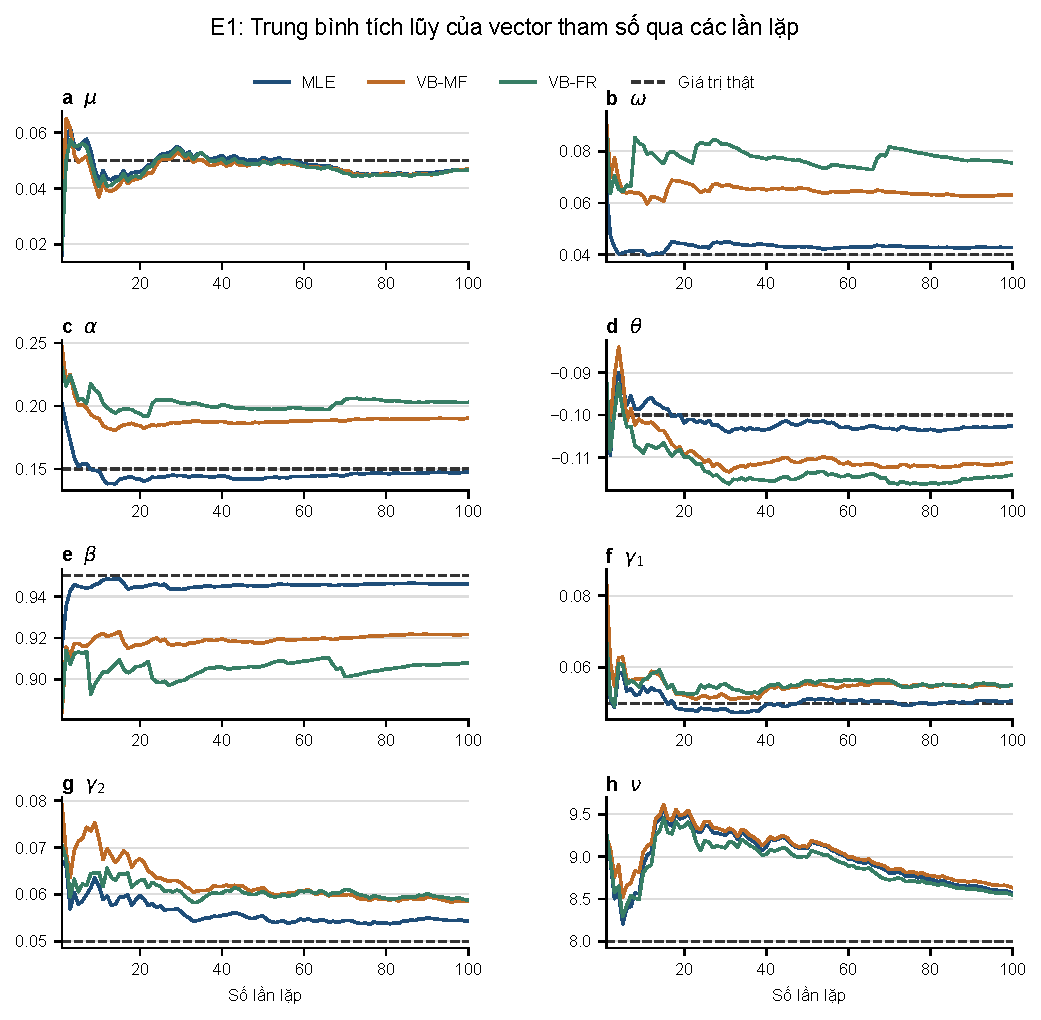
\includegraphics[width=\textwidth]{hinh_tong_hop/vector_E1.pdf}\caption{E1: Trung bình tích lũy $\bar\theta_{j,n}$ của tám tham số EGARCH-X qua các lần lặp. Đường đứt nét là giá trị sinh dữ liệu; mỗi đường dùng đúng các checkpoint của phương pháp tương ứng.}\label{fig:vector-E1}\end{figure}
\subsection{E2: \texorpdfstring{không đòn bẩy, $\theta_0=0$, $\nu_0=8$}{khong don bay, theta0=0, nu0=8}}
Vector tham số sinh dữ liệu $\boldsymbol\theta_0$ được khai báo bằng $\mu=0{,}050$, $\omega=0{,}040$, $\alpha=0{,}150$, $\theta=0{,}000$, $\beta=0{,}950$, $\gamma_1=0{,}050$, $\gamma_2=0{,}050$, $\nu=8{,}000$.
\begin{table}[H]\centering\footnotesize
\caption{E2: Hợp lý cực đại (MLE): khôi phục tham số}\label{tab:E2-mle}
\begin{tabular}{l r r r r r}
\toprule
\textbf{Tham số} & \textbf{Mean} & \textbf{Bias} & \textbf{RMSE} & \textbf{SE} & \textbf{CP 95\%} \\
\midrule
$\mu$ & 0,049 & $-$0,001 & 0,031 & 0,031 & 97\% \\
$\omega$ & 0,044 & 0,004 & 0,016 & 0,016 & 95\% \\
$\alpha$ & 0,149 & $-$0,001 & 0,029 & 0,029 & 95\% \\
$\theta$ & $-$0,001 & $-$0,001 & 0,017 & 0,017 & 97\% \\
$\beta$ & 0,944 & $-$0,006 & 0,019 & 0,018 & 95\% \\
$\gamma_1$ & 0,051 & 0,001 & 0,018 & 0,018 & 93\% \\
$\gamma_2$ & 0,056 & 0,006 & 0,019 & 0,018 & 96\% \\
$\nu$ & 8,572 & 0,572 & 1,643 & 1,540 & 97\% \\
\bottomrule
\end{tabular}
\par\vspace{0.25em}\begin{minipage}{0.95\textwidth}\scriptsize Số lần lặp hợp lệ $N=100$; mỗi chuỗi có $T=2000$ quan sát sau burn-in $=200$. CP 95\% Wald chỉ tính trên 100/100 lần lặp có Hessian xác định dương.\end{minipage}
\end{table}

\begin{table}[H]\centering\footnotesize
\caption{E2: Bayes biến phân mean-field (VB-MF): khôi phục tham số}\label{tab:E2-vb_mean_field}
\begin{tabular}{l r r r r r}
\toprule
\textbf{Tham số} & \textbf{Mean} & \textbf{Bias} & \textbf{RMSE} & \textbf{SE} & \textbf{CP 95\%} \\
\midrule
$\mu$ & 0,048 & $-$0,002 & 0,033 & 0,033 & 96\% \\
$\omega$ & 0,101 & 0,061 & 0,080 & 0,051 & 8\% \\
$\alpha$ & 0,213 & 0,063 & 0,069 & 0,029 & 45\% \\
$\theta$ & 0,000 & 0,000 & 0,021 & 0,021 & 96\% \\
$\beta$ & 0,875 & $-$0,075 & 0,095 & 0,058 & 2\% \\
$\gamma_1$ & 0,059 & 0,009 & 0,025 & 0,024 & 92\% \\
$\gamma_2$ & 0,065 & 0,015 & 0,028 & 0,024 & 89\% \\
$\nu$ & 8,497 & 0,497 & 1,502 & 1,417 & 94\% \\
\bottomrule
\end{tabular}
\par\vspace{0.25em}\begin{minipage}{0.95\textwidth}\scriptsize Số lần lặp hợp lệ $N=100$; mỗi chuỗi có $T=2000$ quan sát sau burn-in $=200$. \end{minipage}
\end{table}

\begin{table}[H]\centering\footnotesize
\caption{E2: Bayes biến phân full-rank (VB-FR): khôi phục tham số}\label{tab:E2-vb_full_rank}
\begin{tabular}{l r r r r r}
\toprule
\textbf{Tham số} & \textbf{Mean} & \textbf{Bias} & \textbf{RMSE} & \textbf{SE} & \textbf{CP 95\%} \\
\midrule
$\mu$ & 0,049 & $-$0,001 & 0,033 & 0,033 & 97\% \\
$\omega$ & 0,109 & 0,069 & 0,092 & 0,061 & 35\% \\
$\alpha$ & 0,219 & 0,069 & 0,083 & 0,046 & 50\% \\
$\theta$ & $-$0,003 & $-$0,003 & 0,023 & 0,023 & 98\% \\
$\beta$ & 0,866 & $-$0,084 & 0,112 & 0,073 & 23\% \\
$\gamma_1$ & 0,059 & 0,009 & 0,026 & 0,024 & 90\% \\
$\gamma_2$ & 0,064 & 0,014 & 0,028 & 0,025 & 90\% \\
$\nu$ & 8,478 & 0,478 & 1,546 & 1,471 & 97\% \\
\bottomrule
\end{tabular}
\par\vspace{0.25em}\begin{minipage}{0.95\textwidth}\scriptsize Số lần lặp hợp lệ $N=100$; mỗi chuỗi có $T=2000$ quan sát sau burn-in $=200$. \end{minipage}
\end{table}

Đối với hệ số đòn bẩy $\theta$, MLE: Mean $=$-$0,0006$, RMSE $=0,0166$; VB-MF: Mean $=$-$0,0001$, RMSE $=0,0209$; VB-FR: Mean $=$-$0,0026$, RMSE $=0,0228$. Hình bên dưới cho thấy toàn bộ đường trung bình tích lũy, qua đó phân biệt sai lệch bền vững với dao động của vài lần lặp đầu.
\begin{figure}[H]\centering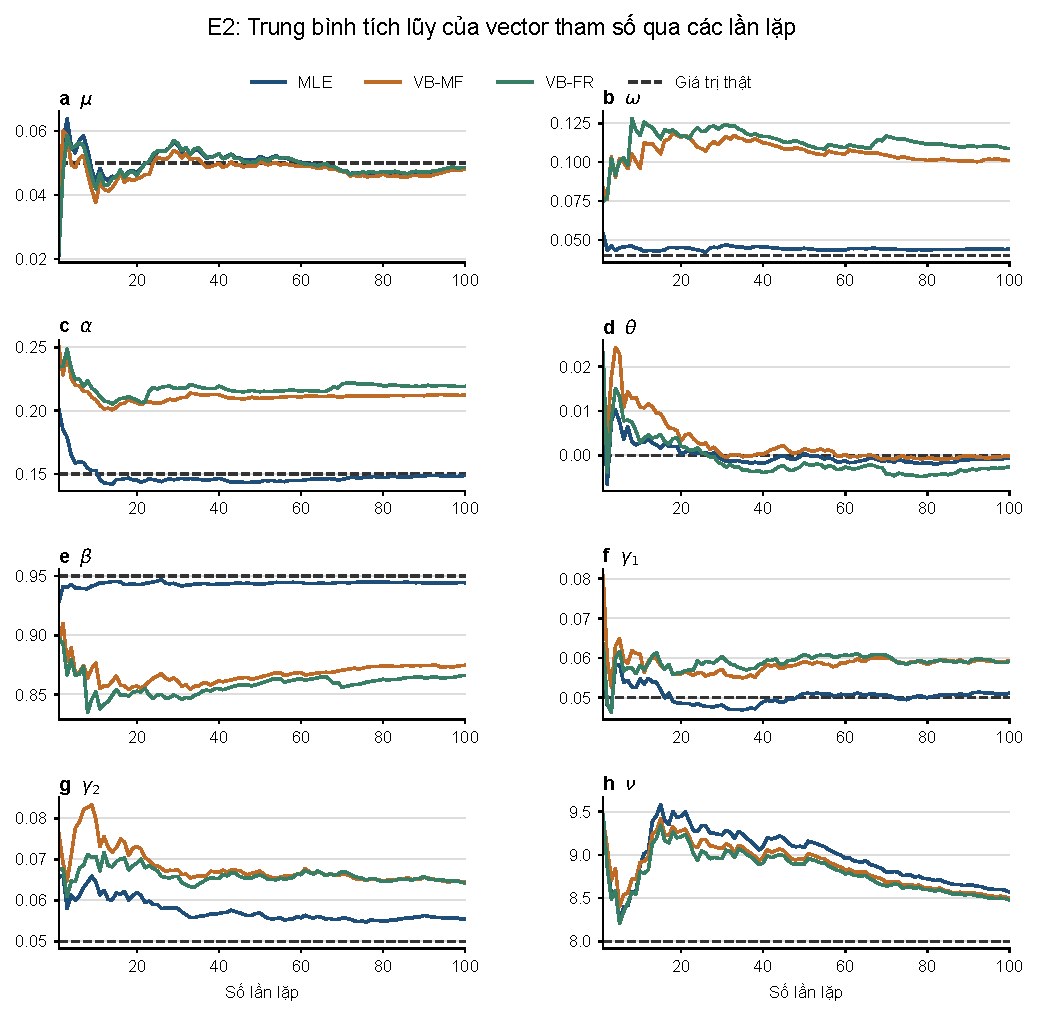
\includegraphics[width=\textwidth]{hinh_tong_hop/vector_E2.pdf}\caption{E2: Trung bình tích lũy $\bar\theta_{j,n}$ của tám tham số EGARCH-X qua các lần lặp. Đường đứt nét là giá trị sinh dữ liệu; mỗi đường dùng đúng các checkpoint của phương pháp tương ứng.}\label{fig:vector-E2}\end{figure}
\subsection{E3: \texorpdfstring{đuôi dày, $\theta_0=-0{,}10$, $\nu_0=4$}{duoi day, theta0=-0,10, nu0=4}}
Vector tham số sinh dữ liệu $\boldsymbol\theta_0$ được khai báo bằng $\mu=0{,}050$, $\omega=0{,}040$, $\alpha=0{,}150$, $\theta=-0{,}100$, $\beta=0{,}950$, $\gamma_1=0{,}050$, $\gamma_2=0{,}050$, $\nu=4{,}000$.
\begin{table}[H]\centering\footnotesize
\caption{E3: Hợp lý cực đại (MLE): khôi phục tham số}\label{tab:E3-mle}
\begin{tabular}{l r r r r r}
\toprule
\textbf{Tham số} & \textbf{Mean} & \textbf{Bias} & \textbf{RMSE} & \textbf{SE} & \textbf{CP 95\%} \\
\midrule
$\mu$ & 0,048 & $-$0,002 & 0,026 & 0,026 & 93\% \\
$\omega$ & 0,043 & 0,003 & 0,013 & 0,012 & 95\% \\
$\alpha$ & 0,146 & $-$0,004 & 0,032 & 0,032 & 89\% \\
$\theta$ & $-$0,103 & $-$0,003 & 0,022 & 0,021 & 95\% \\
$\beta$ & 0,946 & $-$0,004 & 0,015 & 0,014 & 92\% \\
$\gamma_1$ & 0,050 & 0,000 & 0,021 & 0,021 & 92\% \\
$\gamma_2$ & 0,054 & 0,004 & 0,022 & 0,021 & 89\% \\
$\nu$ & 4,121 & 0,121 & 0,435 & 0,418 & 98\% \\
\bottomrule
\end{tabular}
\par\vspace{0.25em}\begin{minipage}{0.95\textwidth}\scriptsize Số lần lặp hợp lệ $N=100$; mỗi chuỗi có $T=2000$ quan sát sau burn-in $=200$. CP 95\% Wald chỉ tính trên 100/100 lần lặp có Hessian xác định dương.\end{minipage}
\end{table}

\begin{table}[H]\centering\footnotesize
\caption{E3: Bayes biến phân mean-field (VB-MF): khôi phục tham số}\label{tab:E3-vb_mean_field}
\begin{tabular}{l r r r r r}
\toprule
\textbf{Tham số} & \textbf{Mean} & \textbf{Bias} & \textbf{RMSE} & \textbf{SE} & \textbf{CP 95\%} \\
\midrule
$\mu$ & 0,047 & $-$0,003 & 0,026 & 0,026 & 94\% \\
$\omega$ & 0,064 & 0,024 & 0,033 & 0,022 & 29\% \\
$\alpha$ & 0,189 & 0,039 & 0,048 & 0,028 & 75\% \\
$\theta$ & $-$0,113 & $-$0,013 & 0,025 & 0,022 & 91\% \\
$\beta$ & 0,919 & $-$0,031 & 0,038 & 0,021 & 12\% \\
$\gamma_1$ & 0,055 & 0,005 & 0,027 & 0,026 & 89\% \\
$\gamma_2$ & 0,059 & 0,009 & 0,026 & 0,025 & 89\% \\
$\nu$ & 4,188 & 0,188 & 0,464 & 0,424 & 83\% \\
\bottomrule
\end{tabular}
\par\vspace{0.25em}\begin{minipage}{0.95\textwidth}\scriptsize Số lần lặp hợp lệ $N=100$; mỗi chuỗi có $T=2000$ quan sát sau burn-in $=200$. \end{minipage}
\end{table}

\begin{table}[H]\centering\footnotesize
\caption{E3: Bayes biến phân full-rank (VB-FR): khôi phục tham số}\label{tab:E3-vb_full_rank}
\begin{tabular}{l r r r r r}
\toprule
\textbf{Tham số} & \textbf{Mean} & \textbf{Bias} & \textbf{RMSE} & \textbf{SE} & \textbf{CP 95\%} \\
\midrule
$\mu$ & 0,047 & $-$0,003 & 0,027 & 0,027 & 94\% \\
$\omega$ & 0,076 & 0,036 & 0,054 & 0,040 & 69\% \\
$\alpha$ & 0,201 & 0,051 & 0,069 & 0,046 & 71\% \\
$\theta$ & $-$0,117 & $-$0,017 & 0,029 & 0,023 & 96\% \\
$\beta$ & 0,905 & $-$0,045 & 0,071 & 0,055 & 49\% \\
$\gamma_1$ & 0,055 & 0,005 & 0,026 & 0,026 & 90\% \\
$\gamma_2$ & 0,060 & 0,010 & 0,029 & 0,027 & 90\% \\
$\nu$ & 4,131 & 0,131 & 0,466 & 0,447 & 92\% \\
\bottomrule
\end{tabular}
\par\vspace{0.25em}\begin{minipage}{0.95\textwidth}\scriptsize Số lần lặp hợp lệ $N=100$; mỗi chuỗi có $T=2000$ quan sát sau burn-in $=200$. \end{minipage}
\end{table}

Đối với hệ số đòn bẩy $\theta$, MLE: Mean $=$-$0,1031$, RMSE $=0,0216$; VB-MF: Mean $=$-$0,1128$, RMSE $=0,0253$; VB-FR: Mean $=$-$0,1165$, RMSE $=0,0286$. Hình bên dưới cho thấy toàn bộ đường trung bình tích lũy, qua đó phân biệt sai lệch bền vững với dao động của vài lần lặp đầu.
\begin{figure}[H]\centering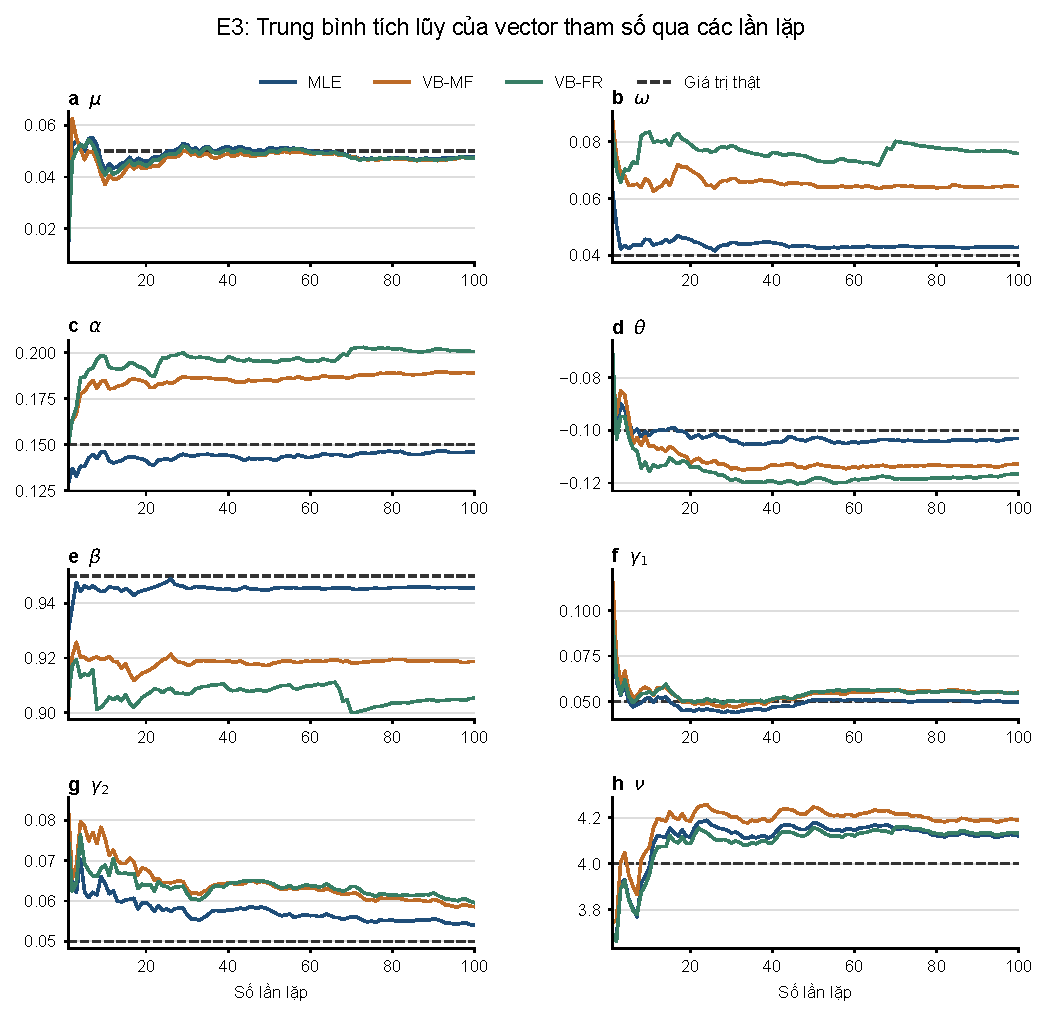
\includegraphics[width=\textwidth]{hinh_tong_hop/vector_E3.pdf}\caption{E3: Trung bình tích lũy $\bar\theta_{j,n}$ của tám tham số EGARCH-X qua các lần lặp. Đường đứt nét là giá trị sinh dữ liệu; mỗi đường dùng đúng các checkpoint của phương pháp tương ứng.}\label{fig:vector-E3}\end{figure}
\section{MCMC trên EGARCH-X Student-$t$}
NUTS đạt $\max\hat R=1,0125$, ESS nhỏ nhất 1340 và không có phân kỳ. Khoảng hậu nghiệm 95\% của hệ số đòn bẩy $\theta$ loại trừ 0, phù hợp với tác động bất đối xứng của cú sốc lên log-phương sai. So với MCMC, VB-MF báo độ lệch chuẩn hậu nghiệm của $\omega$ và $\beta$ lần lượt bằng 0,37 và 0,29 lần; VB-FR đạt khoảng 0,75 lần cho cả hai. Tâm hậu nghiệm gần nhau không đồng nghĩa với mức bất định được hiệu chỉnh tốt.

\begin{table}[H]\centering\normalsize
\caption{Hậu nghiệm MCMC trên EGARCH-X Student-$t$ và nghiệm MLE đối chiếu}\label{tab:b3-mcmc}
\begin{tabular}{l r r r c}
\toprule
\textbf{Tham số} & \textbf{MLE} & \textbf{TB hậu nghiệm} & \textbf{SD} & \textbf{KTC 95\%} \\
\midrule
$\mu$ & 0,0796 & 0,0800 & 0,0231 & [0,0336; 0,1226] \\
$\omega$ & 0,1599 & 0,1870 & 0,0472 & [0,1093; 0,2948] \\
$\alpha$ & 0,0721 & 0,1121 & 0,0463 & [0,0268; 0,2110] \\
$\theta$ & $-$0,1452 & $-$0,1399 & 0,0362 & [$-$0,2125; $-$0,0710] \\
$\beta$ & 0,6832 & 0,6393 & 0,0691 & [0,4912; 0,7562] \\
$\gamma_1$ & $-$0,0692 & $-$0,0765 & 0,0231 & [$-$0,1268; $-$0,0370] \\
$\gamma_2$ & 0,2986 & 0,3324 & 0,0659 & [0,2167; 0,4715] \\
$\nu$ & 4,2910 & 4,3644 & 0,4809 & [3,5544; 5,4315] \\
\bottomrule
\end{tabular}
\par\vspace{0.25em}\begin{minipage}{0.95\textwidth}\scriptsize Dữ liệu huấn luyện $T=1735$; NUTS: 4 chuỗi, mỗi chuỗi 1.000 vòng warmup và 400 mẫu giữ lại; $\max\hat R=1,0125$, ESS nhỏ nhất $=1340$, 0 phân kỳ, thời gian 8.1 giờ.\end{minipage}
\end{table}
\begin{table}[H]\centering\normalsize
\caption{Bước 3: $R_{sd}=\mathrm{sd}_{\text{VB}}/\mathrm{sd}_{\text{MCMC}}$ (độ lệch chuẩn hậu nghiệm VB so với MCMC, cùng dữ liệu)}\label{tab:b3-rsd}
\begin{tabular}{l r r r}
\toprule
\textbf{Tham số} & $\mathrm{sd}_{\text{MCMC}}$ & $R_{sd}$ VB-MF & $R_{sd}$ VB-FR \\
\midrule
$\mu$ & 0,0231 & 0,95 & 0,94 \\
$\omega$ & 0,0472 & 0,37 & 0,75 \\
$\alpha$ & 0,0463 & 0,88 & 1,01 \\
$\theta$ & 0,0362 & 0,92 & 1,00 \\
$\beta$ & 0,0691 & 0,29 & 0,75 \\
$\gamma_1$ & 0,0231 & 0,82 & 0,86 \\
$\gamma_2$ & 0,0659 & 0,28 & 0,82 \\
$\nu$ & 0,4809 & 0,63 & 0,97 \\
\bottomrule
\end{tabular}
\end{table}

\section{Tổng hợp thứ hạng RMSE}
\begin{table}[H]\centering\normalsize
\caption{Số tham số EGARCH-X mà mỗi phương pháp đạt RMSE nhỏ nhất, theo trường hợp E1-E3.}\label{tab:dem-thang}
\begin{tabular}{l r l r r r}
\toprule
\textbf{Trường hợp} & \textbf{Số tham số} & $B$ (MLE/MF/FR) & \textbf{MLE} & \textbf{VB-MF} & \textbf{VB-FR} \\
\midrule
E1 & 8 & 100/100/100 & 6 & 2 & 0 \\
E2 & 8 & 100/100/100 & 7 & 1 & 0 \\
E3 & 8 & 100/100/100 & 7 & 1 & 0 \\
\bottomrule
\end{tabular}
\end{table}


\section{Kết luận và giới hạn diễn giải}
Trên mẫu VN30F1M được khảo sát, EGARCH-X Student-$t$ với MLE đạt AIC,
BIC, QLIKE và NLS thấp nhất trong sáu mô hình một trạng thái được so sánh.
Phân phối đuôi dày và biến ngoại sinh có đóng góp trong những đối chiếu
hiện có. NUTS trên mô hình EGARCH-X Student-$t$
hội tụ và cho thấy hiệu ứng đòn bẩy âm; VB mean-field đánh giá thấp độ phân
tán hậu nghiệm của một số hệ số dai dẳng. Những kết luận này giới hạn ở
chuỗi VN30F1M, sáu đặc tả và cách chia mẫu đã dùng.

Mô phỏng EGARCH-X Student-$t$ ở ba trường hợp E1-E3 đánh giá khả năng khôi
phục tham số, nhưng không thay thế kiểm chứng ngoài mẫu trên dữ liệu khác.
Chuỗi hợp đồng liên tục do nhà cung cấp ghép sẵn nên nghiên cứu chưa tách
riêng được ảnh hưởng của ngày chuyển hợp đồng lên các quan sát cực trị.

\end{document}
